\chapter{圆锥曲线}
远在古希腊时代,人们就开始研究一个平面和一个正瞬
锥的截线的性质,并且获得了丰硕的成果,这些截线分别有
椭圆、抛物线和双曲线,并统称为圆锥曲线,在第二章
附录里,我们已用球面切线长相等原理证明了它们分别具有
如下几何特征。

椭圆有两个焦点$F_1,F_2$, 对椭圆上任一点$P$有
\[\overline{PF_1}+\overline{PF_2}=\text{常数}\]

双曲线有两个焦点$F_1,F_2$, 对双曲线上任一点$P$有
\[\overline{PF_1}-\overline{PF_2}=\text{常数}\]

抛物线有一个焦点,对抛物线上任一点$P$到焦点$F$与到
一定直线$\ell$的距离$d$相等,即
\[\overline{PF}:d=1\]

这一章,我们将要根据上述圆锥曲线的几何特性来定义
椭圆、双曲线和抛物线,建立它们在平面直角坐标系中的标
准方程,并利用标准方程进一步研究圆锥曲线其它的几何特
性。

\section{圆锥曲线的标准方程及其性质}
\subsection{椭圆的标准方程和形状}
\begin{blk}
    {定义} 平面内与两定点的距离之和等于常数(这常数必
须大于两定点间的距离)的点的轨迹叫做椭圆。这两定点叫
做椭圆的\textbf{焦点}。两焦点间的距离叫做\textbf{焦距}。
\end{blk}

下面,我们根据椭圆的定义来建立椭圆的方程。

设$F_1$、$F_2$是椭圆的两个焦点,取射线$F_1F_2$作为$X$轴
的正半轴,$\overline{F_1F_2}$的垂直平分线作为$Y$轴(图6.1)。设
焦距$\overline{F_1F_2}=2c\; (c>0)$,则
\[F_1(-c,0),\qquad F_2(c,0)\]

\begin{figure}[htp]
    \centering
    \begin{tikzpicture}[>=latex]
\draw[->](-2.5,0)--(2.5,0)node[right]{$X$};
\draw[->](0,-2)--(0,2)node[right]{$Y$};
\draw[thick](0,0) ellipse [x radius=2, y radius=1.25];        
\tkzDefPoints{-1.56/0/F_1, 1.56/0/F_2, 1/1.08/P}
\tkzDrawSegments[thick](F_1,P P,F_2)
\tkzLabelPoints[below](F_1,F_2)
\tkzLabelPoints[above](P)
\node at (0,0)[below left]{$O$};
    \end{tikzpicture}
    \caption{}
\end{figure}


设$P(x,y)$是椭圆上的任一点,
它到$F_1$、$F_2$的距离之和等于常数
$2a\; (a>0)$, 则
\[\overline{PF_1}+\overline{PF_2}=2a\]
由求两点的距离公式得
\[\sqrt{(x+c)^2+y^2}+\sqrt{(x-c)^2+y^2}=2a\]
去根号,整理得
\begin{equation}
    (a^2-c^2)x^2+a^2y^2=a^2(a^2-c^2)
\end{equation}
因$\overline{PF_1}+\overline{PF_2}>\overline{F_1F_2}$, 所以$a>c,\; a^2-c^2>0$, 
设$a^2-c^2=b^2\; (b>0)$, 代入(6.1)式得
\[b^2x^2+a^2y^2=a^2b^2\]
两边同除$a^2b^2$得
\begin{equation}
 \boxed{\frac{x^2}{a^2}+\frac{y^2}{b^2}=1}   
\end{equation}
这就是说,椭圆上任一点的坐标都满足方程(6.2); 反过来,
设$P(x_1,y_1)$的坐标满足方程(6.2), 则
\[\frac{x_1^2}{a^2}+\frac{y_1^2}{b^2}=1\]
\[y^2_1=b^2\left(1-\frac{x^2_1}{a^2}\right)=(a^2-c^2)\left(1-\frac{x^2_1}{a^2}\right)\]
于是
\[\begin{split}
    \overline{PF_1}&=\sqrt{(x_1+c)^2+y^2_1}\\
    &=\sqrt{(x_1+c)^2+(a^2-c^2)\left(1-\frac{x^2_1}{a^2}\right)}\\
    &=\sqrt{a^2+2cx_1+\frac{c^2}{a^2}x^2_1}\\
    &=\left|a+\frac{c}{a}x_1\right|
\end{split}\]
由$\frac{x_1^2}{a^2}+\frac{y_1^2}{b^2}=1$,可推知
$\frac{x_1^2}{a^2}\le 1$,$|x_1|\le a$。

又因$c<a$,所以$\frac{c}{a}<1$,$\left|\frac{c}{a}x_1\right|<a$
,$a+\frac{c}{a}x_1>0$,因此:
\begin{equation}
    \overline{PF_1}=a+\frac{c}{a}x_1
\end{equation}
同理可证,
\[\overline{PF_2}=a-\frac{c}{a}x_1\]
所以:$\overline{PF_1}+\overline{PF_2}=2a$

这就是说,坐标满足方程(6.2)的点$P$也一定在椭圆上,由以
上证明,所以方程(6.2)是所求的椭圆方程,并把方程(6.2)
叫做\textbf{椭圆的标准方程}。

下面,用椭圆的标准方程来研究椭圆的几何形状。

首先,由于方程(6.2)中只含有$x,y$的平方,故把一
个坐标变号,对于方程没有影响,这就表明:如果$M(x,y)$
在椭圆上,那么,$M_1(x,-y)$, $M_2(-x,-y)$, $M_3(-x,
y)$各点也都在椭圆上,所以椭圆既是以$X$轴或$Y$轴为对称轴的
轴对称图形,又是以坐标原点为对称中心的中心对称图形,对
称中心又叫做椭圆的中心。

其次,由方程(6.2)得
\[\frac{x^2}{a^2}\le 1,\qquad \frac{y^2}{b^2}\le 1\]
\[-a\le x\le a,\qquad -b\le y\le b\]
这两个不等式表明椭圆全部包含在如图6.2所示的长方形
内。

最后,我们来讨论椭圆在第
I象限内的性态。由(6.2)得
\[y=\pm\frac{b}{a}\sqrt{a^2-x^2}\]
在第I象限,椭圆方程可写为
\[y=\frac{b}{a}\sqrt{a^2-x^2},\qquad 0\le x\le a\]
当$x=0$时,$y=b$, 当$x$递增时,
$y$递减,当$x=a$时,$y=0$, 
因此椭圆在第I象限内的轨迹大致是$B_2A_2$这部分曲线,由
对称性可画出整个椭圆的图象(图6.2)。

\begin{figure}[htp]
    \centering
    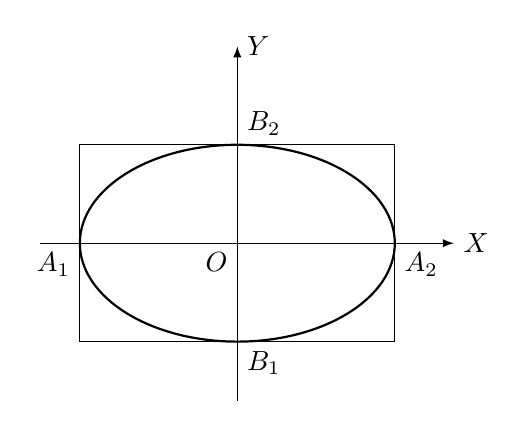
\begin{tikzpicture}[>=latex]
\draw[->](-2.5,0)--(2.75,0)node[right]{$X$};
\draw[->](0,-2)--(0,2.5)node[right]{$Y$};
\draw[thick](0,0) ellipse [x radius=2, y radius=1.25];        
\node at (0,0)[below left]{$O$};
\draw(-2,-1.25) rectangle (2,1.25);
\node at (-2,0)[below left]{$A_1$};
\node at (2,0)[below right]{$A_2$};
\node at (0,1.25)[above right]{$B_2$};
\node at (0,-1.25)[below right]{$B_1$};
\tkzDrawPoint(1.5,0)\tkzDrawPoint(-1.5,0)
    \end{tikzpicture}
    \caption{}
\end{figure}

当$y=0$, $x=\pm a$, 点$A_1(-a,0)$, $A_2(+a,0)$
是$X$轴上距$Y$轴最远的两个点,当$x=0$, $y=\pm b$, 点
$B_1(0,-b)$, $B_2(0,+b)$是$Y$轴上距$X$轴距离最远的
两个点,这四点,$A_1$、$A_2$、$B_1$、$B_2$叫做\textbf{椭圆的顶点}。
$\overline{A_1A_2},\overline{B_1B_2}$分别叫做椭圆的长和轴短轴。$\overline{A_1A_2}=2a$, 
$\overline{B_1B_2}=2b$, $a$和$b$分别叫做椭圆的\textbf{长半轴长和短半轴长}。
长轴和短轴的交点叫做\textbf{椭圆的中心}。

如果$a=b$, 那么方程(6.2)化为
\[x^2+y^2=a^2\]
这时椭圆成为圆,$c=\sqrt{a^2-b^2}=0$, 即椭圆的两个焦点重
合于圆心,因此可以说\textbf{圆是椭圆的特殊情形}。

由以上讨论可以看出,椭圆的形状依赖于$a$和$b$, 数量
$c=\sqrt{a^2-b^2}$可表示出椭圆离开圆的偏差。由$c^2=a^2-b^2$
可得
\[\frac{c}{a}=\sqrt{1-\left(\frac{b}{a}\right)^2},\qquad \frac{b}{a}=\sqrt{1-\left(\frac{c}{a}\right)^2}\]
比值
\[e=\frac{c}{a}=\frac{\sqrt{a^2-b^2}}{a}\]
叫做\textbf{椭圆的离心率},用它可同样来表出椭圆的形状。由$c<
a$, 可知$e<1$, 当离心率愈来愈大时,也就是愈来愈接近
1时,$1-e^2$就越小,椭圆的形状就愈扁平;反之,就愈接
近于圆,当$e=0$时,$a=b$椭圆就成为圆了。

如果椭圆的中心在原点,焦点在$Y$轴上,那么长轴也-
定在$Y$轴上,这时两个焦点$F_1,F_2$的坐标分别是$(0,-c)$,
$(0,c)$ (图6.3), 求得圆的标准方程是
\begin{equation}
    \boxed{\frac{x^2}{b^2}+\frac{y^2}{a^2}=1}\qquad a\ge b>0
\end{equation}
把方程(6.2)的变量$x$和$y$互换就可得到方程(6.6).

\begin{figure}[htp]\centering
    \centering
\begin{tikzpicture}[>=latex, scale=1]
    \draw[->](-1.5,0)--(1.75,0)node[right]{$X$};
    \draw[->](0,-2)--(0,2.5)node[right]{$Y$};
    \draw[thick](0,0) ellipse [x radius=.7, y radius=1.5];  
    \tkzDefPoints{0/-1.2/F_1, 0/1.2/F_2}
\tkzLabelPoints[right](F_1,F_2)
\tkzDrawPoints(F_1,F_2)
\node at (0,0)[below left]{$O$}; 
\node at (0,1.5)[above right]{$B(0,a)$}; 
\node at (0.7,0)[below right]{$A(b,0)$}; 
    \end{tikzpicture}
    \caption{}
    \end{figure}


\begin{example}
    已知椭圆的长轴长是10, 焦距是8, 求椭圆的标准方程。
\end{example}

\begin{solution}
    由已知条件得$2a=10,\quad 2c=8$,所以:
\[a=5,\qquad c=4,\qquad b^2=a^2-c^2=5^2-4^2=9\]
因此所求椭圆的标准方程为
\[\frac{x^2}{25}+\frac{y^2}{9}=1\]
\end{solution}

\begin{example}
    求椭圆$4x^2+9y^2=36$的长轴、短轴长、离心率、
焦点和顶点的坐标,并用描点法画出它的图形。
\end{example}

\begin{solution}
    已知方程可化为
    \[\frac{x^2}{9}+\frac{y^2}{4}=1\]
这是长轴在$X$轴上,中心在坐标原点的椭圆标准方程。
因此$a=3$, $b=2$, $c=\sqrt{3^2-2^2}=\sqrt{5}$, 顶点$A'(-3,
0)$, $A(3,0)$, $B'(0,-2)$, $B(0,2)$. 焦点
$F_1(-\sqrt{5},0)$, $F_2(\sqrt{5},0)$. 离心率$e=\frac{c}{a}=\frac{\sqrt{5}}{3}$。

在第I象限已知椭圆方程可写为
\[y=\frac{2}{3}\sqrt{9-x^2},\qquad 0\le x\le 3\]
算出一些满足所求椭圆方程的点的坐标$(x,y)$:
\begin{center}
    \begin{tabular}{cccccccc}
\hline
$x$&0&0.5&1&1.5&2&2.5&3\\
\hline
$y$&2&1.97&1.89&1.73&1.49&1.11&0\\
\hline
    \end{tabular}
\end{center}
描点画出椭圆在第I象限的图
象,然后根据椭圆的对称性就可
画出整个椭圆的图象(图6.4)。
\end{solution}

\begin{figure}[htp]\centering
    \begin{minipage}[t]{0.48\textwidth}
    \centering
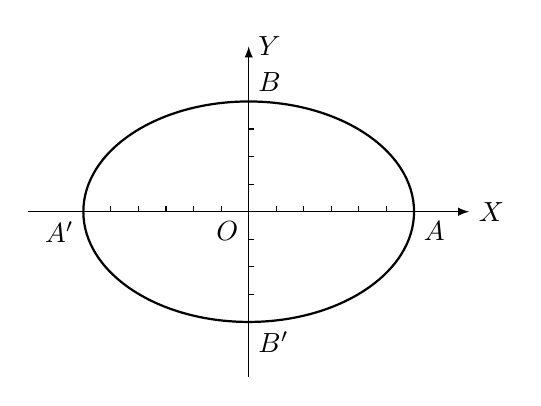
\begin{tikzpicture}[>=latex, scale=.7]
    \draw[->](-4,0)--(4,0)node[right]{$X$};
    \draw[->](0,-3)--(0,3)node[right]{$Y$};
    \draw[thick](0,0)node[below left]{$O$} ellipse [x radius=3, y radius=2];  
    \node at (-3,0)[below left]{$A'$};
    \node at (3,0)[below right]{$A$};
    \node at (0,2)[above right]{$B$};
    \node at (0,-2)[below right]{$B'$};
\tkzDefPoints{0/2/A, .5/1.97/B, 1/1.89/C, 1.5/1.73/D, 2/1.49/E, 2.5/1.11/F, 3/0/G}
\tkzDrawPoints(A,B,C,D,E,F,G)

\tkzDefPoints{0/-2/A, .5/-1.97/B, 1/-1.89/C, 1.5/-1.73/D, 2/-1.49/E, 2.5/-1.11/F, 3/0/G}
\tkzDrawPoints(A,B,C,D,E,F,G)

\tkzDefPoints{0/2/A, -.5/1.97/B, -1/1.89/C, -1.5/1.73/D, -2/1.49/E, -2.5/1.11/F, -3/0/G}
\tkzDrawPoints(A,B,C,D,E,F,G)

\tkzDefPoints{0/-2/A, -.5/-1.97/B, -1/-1.89/C, -1.5/-1.73/D, -2/-1.49/E, -2.5/-1.11/F, -3/0/G}
\tkzDrawPoints(A,B,C,D,E,F,G)

\foreach \x in {-2.5,-2,...,2.5}
{
    \draw(\x,0)--(\x,.1);
}
\foreach \x in {-1.5,-1,...,1.5}
{
    \draw(0,\x)--(.1,\x);
}
    \end{tikzpicture}
    \caption{}
    \end{minipage}
    \begin{minipage}[t]{0.48\textwidth}
    \centering
    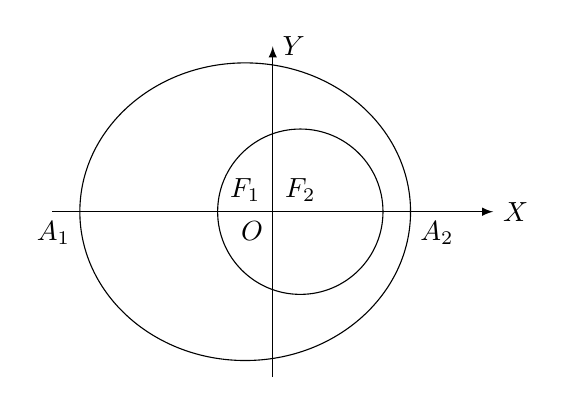
\begin{tikzpicture}[>=latex, scale=.7]
        \draw[->](-4,0)--(4,0)node[right]{$X$};
        \draw[->](0,-3)--(0,3)node[right]{$Y$};
    \draw(.5,0)node[above]{$F_2$} circle(1.5);
    \draw(-.5,0)node[above]{$F_1$} ellipse[x radius= 3,  y radius= 2.7];
    \tkzDrawPoint(.5,0)\tkzDrawPoint(-.5,0)
    \node at (0,0) [below left]{$O$};
    \node at (2.5,0) [below right]{$A_2$};
    \node at (-3.5,0) [below left]{$A_1$};
    \end{tikzpicture}
    \caption{}
    \end{minipage}
    \end{figure}


\begin{example}
    我国第一颗人造地球
卫星的运行轨道是以地球中心为
一焦点的椭圆,卫星的近地点与
地球表面距离为439公里;远地点
与地球表面距离为2384公里,已知地球半径约为6371公里,
试求卫星轨道的近似方程及其离心率。
\end{example}


\begin{solution}
    设地球中心$F_2$在$X$轴上(图6.5),所求方程为
\[\frac{x^2}{a^2}+\frac{y^2}{b^2}=1\]
依题意
\[\begin{split}
    \overline{A_1F_2}&=a+c=6371+2284=8755\\
    \overline{A_2F_2}&=a-c=6371+439=6810
\end{split}\]
由以上两式联立求解得
\[a=7782.5,\qquad c=972.5,\qquad b=\sqrt{a^2-c^2}=7721.5\]
所以,所求卫星轨道的近似方程为
\[\frac{x^2}{(7782.5)^2}+\frac{y^2}{(7721.5)^2}=1\]
其离心率
$e=\frac{c}{a}\approx 0.125$
\end{solution}

\begin{ex}
\begin{enumerate}
    \item 已知椭圆的长轴长是6, 短轴长是2, 焦点在$X$轴上,
    求这椭圆的标准方程并画出这椭圆的草图。
    \item 在第1题中,若焦点在$Y$轴,椭圆的标准方程为何?
    \item 已知椭圆的一个焦点是$F_1(-3,0)$与$X$轴一个交点
    $A(4,0)$, 求此椭圆的方程。
    \item 求以下椭圆的长轴长,短轴长、焦点的坐标及其离心率。
\begin{multicols}{2}
\begin{enumerate}
    \item $\frac{x^2}{100}+\frac{y^2}{36}=1$
    \item $25x^2+9y^2=100$
    \item $\frac{x^2}{16}+\frac{y^2}{64}=1$
    \item $49x^2+9y^2=2500$
\end{enumerate}
\end{multicols}

\item 已知椭圆中心在原点,一焦点是$F(3,0)$, 椭圆与$X$
轴相交于$A$、$A'$两点,$\overline{AF}=2$, $\overline{A'F}=8$, 求此椭圆的方程。
\item 已知地球的轨道是一个椭圆,太阳在它的一个焦点上,
长轴长约30亿公里,离心率$e=1/60$, 
求地球的轨道方程,地球的轨道中心与太阳的距离,以及近日点,远日
点到太阳的距离。
\item 试求平分圆$x^2+y^2=25$上各点的纵坐标,而横坐标不
变的点的轨迹方程。
\item 试求把圆$x^2+y^2=100$上各纵坐标分为2:3, 而横
坐标不变的点的轨迹方程。
\item 一动点与直线$x=8$的距离是它与点$(2,0)$的距离的
2倍,求这动点的轨迹方程。
\item 一定长为$a$的线段,两端在互相垂直的二直线上移动,
试求此线段上任意一点的轨迹方程。
\item 设一三角形的一边的两个端点为$(0,6)$, $(0,-6)$,其它两
边斜率的乘积是$-\frac{4}{9}$,
试求另一顶点的轨迹。
\item 已知$A>0$, $B>0$, 且$A<B$, 试求椭圆$Ax^2+By^2
=C$的焦点坐标。
\item 试证:椭圆的短半轴长是其中一焦点到长轴两顶点距离
的比例中项。
\item 在椭圆$\frac{x^2}{45}+\frac{y^2}{20}=1$上求一点,使它与两焦点连线互相垂直。
\end{enumerate}
\end{ex}

\subsection{双曲线的标准方程和形状}
\begin{blk}
    {定义} 平面内到两定点距离的差的绝对值等于常数(常
数小于两定点间的距离)的轨迹叫做双曲线。这两个定点叫
做双曲线的焦点,两个焦点间的距离叫做焦距。
\end{blk}

根据双曲线的定义,我们来求它的方程:









\begin{example}
    
\end{example}

\begin{solution}
    
\end{solution}

\begin{example}
    
\end{example}



\begin{solution}
    
\end{solution}

\begin{example}
    
\end{example}



\begin{solution}
    
\end{solution}

\begin{example}
    
\end{example}



\begin{solution}
    
\end{solution}

\begin{example}
    
\end{example}



\begin{solution}
    
\end{solution}

\begin{example}
    
\end{example}



\begin{solution}
    
\end{solution}

\begin{example}
    
\end{example}



\begin{solution}
    
\end{solution}




















\begin{ex}
\begin{enumerate}
    \item 对双曲线和抛物线情况证明本节定理。
    \item 已知椭圆$3x^2+4y^2=12$, 求倾角为$135^{\circ}$的椭圆平行弦
    中点所在的直线方程。
    \item 已知双曲线$2x^2-y^2=6$, 它的一族平行弦的倾角是
    $30^{\circ}$, 求这族平行弦中点所在的直线方程。
    \item 在练习2、3中写出与弦平行的直径和它的共轭直径的
    方程。
    \item 已知抛物线$y^2=6x$的一族平行弦的斜率是$1/2$, 
    求平分这族平行弦的直径方程。
    \item 设$P_0(x_0,y_0)$是双曲线
    $\frac{x^2}{a^2}-\frac{y^2}{b^2}=1$
    与它的一条直
    径$y=kx$的交点,求证:双曲线在$P_0(x_0,y_0)$的切线
    平行于这条直径的共轭直径。
\end{enumerate}
\end{ex}

\subsection*{习题6.1}
\begin{enumerate}
\item 在椭圆$24x^2+30y^2=720$上,求与短轴相距为5的点
的坐标。
\item 一椭圆以坐标轴为对称轴,坐标原点为对称中心且经过
点$M(\sqrt{3},-2)$, $N(-2\sqrt{3},1)$, 求此椭圆的方
程。
\item 点$P(x_1,y_1)$和点$Q(x_2,y_2)$分别位于椭圆的内部
和外部,求证
\[\frac{x_1^2}{a^2}+\frac{y_1^2}{b^2}<1,\qquad \frac{x_2^2}{a^2}+\frac{y_2^2}{b^2}>1\]
\item 已知一椭圆的准线方程是$x=\pm 8$, 短轴长等于8, 求
此椭圆的方程。
\item 已知椭圆$36x^2+100y^2=3600$, 在它上面求一点使这点
到右焦点的距离是这点到左焦点距离的4倍。
\item 已知椭圆中心在原点,它的一个焦点是$F_2(3,0)$, 求
其上一点$M(4,2.4)$到准线的距离。
\item 求下列各双曲线标准方程。
\begin{enumerate}
\item 两焦点间的距离是8, 两准线间的距离是6;
\item 已知两条准线方程是$x=\pm 3\sqrt{2}$, 两条渐近线的
夹角是直角。
\item 已知渐近线方程是$y=\pm 2x$, 两个焦点距中心的距
离是5.
\item 已知渐近线方程是$y=\pm \frac{5}{3}x$, 且双曲线通过点
$N(6,9)$.
\end{enumerate}

\item 根据下列已知条件,求双曲线$\frac{x^2}{a^2}-\frac{y^2}{b^2}=1$的渐近线
方程。
\begin{enumerate}
    \item 离心率$e=2$; 
    \item 两焦点间的距离是二准线间距离的2倍。
\end{enumerate}

\item 根据下列已知条件,求双曲线$\frac{x^2}{a^2}-\frac{y^2}{b^2}=1$的离心率。
\begin{enumerate}
    \item 两渐近线之间的夹角是$60^{\circ}$;
    \item 两渐近线之间的夹角是$90^{\circ}$.
\end{enumerate}

\item 已知等轴双曲线$x^2-y^2=8$, 求一抛物线方程使它与
已知双曲线有公共焦点且通过点$M(-5,3)$.
\item 通过点$A(2,-5)$引直线平行于双曲线$x^2-4y^2=4$的
渐近线,求此直线的方程。

\item 通过点$A(3,-1)$作双曲线$\frac{x^2}{4}-y^2=1$的弦且被$A$点
平分,求此弦的方程。
\item 求下列抛物线方程,已知
\begin{enumerate}
    \item 顶点在$(0,0)$, 焦点在$(2,0)$;
    \item 顶点在$(0,0)$, 准线是$2x+5=0$;
    \item 顶点在$(0,0)$, 准线是$2y-1=0$;
    \item 顶点在$(0,0)$, 焦点在$(0,-3/5)$.
\end{enumerate}

\item 一条抛物线顶点在原点,它的轴是$X$轴并且它通过点
$M(-1,1)$, 求它的方程。

\item 求椭圆$\frac{x^2}{6}+\frac{y^2}{3}=1$的内接正方形每边所在直线的方程。
\item 求直线$Ax+By+C=0$与椭圆$\frac{x^2}{a^2}+\frac{y^2}{b^2}=1$相切的条
件。

\item 已知椭圆$\frac{x^2}{25}-\frac{y^2}{9}=1$
的两个焦点到它的某条切线的距离之比是9, 求此切线方程。
\item 求双曲线$\frac{x^2}{8}-\frac{y^2}{9}=1$在下列各点的切线,$(2\sqrt{2},0)$, $(-4,3)$.
\item 一条双曲线在点$M(4,2)$与直线$x-y-2=0$相切.
求此双曲线的方程。
\item 求直线:$Ax+By+C=0$与双曲线
$\frac{x^2}{a^2}-\frac{y^2}{b^2}=1$相切
的条件。
\item 已知抛物线$y^2=12x$, 根据下列各条件,求它的切线方
程。
\begin{enumerate}
\item 切点的横坐标$x=3$;
\item 平行于直线$3x-y+5=0$;
\item 垂直于直线$2x+y-7=0$;
\item 与直线$4x-2y+9=0$交成$\pi/4$角。
\end{enumerate}

\item 求直线$y=kx+b$与抛物线$y^2=2px$相切的条件。
\item 直线$x+y=1$与椭圆相交于$C$和$D$两点,求弦$\overline{CD}$的
中点的坐标。
\item 已知椭圆$\frac{x^2}{a^2}+\frac{y^2}{b^2}=1$, 在其上一点$P$的切线和法线分
别与$X$轴相交于$T$点和$G$点,过焦点$F_1$、$F_2$和原点分
别作切线的垂线,设垂足分别为$V$、$U$、$K$, 过$P$点作
$X$轴的垂线,设垂足为$N$, 求证:
\begin{enumerate}
    \item $\overline{ON}\cdot \overline{OT}=a^2$
    \item $\overline{PG}\cdot \overline{OK}=b^2$
    \item $\overline{OG}=e^2\cdot \overline{ON}$
    \item $\overline{F_1V}\cdot  \overline{F_2U}=b^2$
\end{enumerate}
\end{enumerate}


\section{坐标变换}
\subsection{坐标轴的平移}
不改变坐标轴的方向和长度单位,只变换原点的位置,
这种坐标系的变换叫做\textbf{坐标轴的平移},简称\textbf{移轴}。

给定一坐标系$OXY$, 平移
坐标轴得到新坐标系$O'X'Y'$, 
下面我们来确定平面上任意一点
$P$的新坐标$(x',y')$与原坐标
$(x,y)$之间的关系(图6.27)。















































































\begin{ex}
\begin{enumerate}
    \item 试判别下列方程的类型
\begin{enumerate}
\item $16x^2-24xy+9y^2-38x-34y+71=0$
\item $x^2-5xy+13y^2-3x+21y=0$
\item $8x^2+8xy-7y^2+36y+36=0$
\item $4x^2+9y^2-16x-18y-11=0$
\item $2x^2+5xy-3y^2+3x+16y-5=0$
\end{enumerate}

    \item 判别下列方程的类型,并画出它们的图形
\begin{enumerate}
\item $5x^2-6xy+5y^2-4x-4y-4=0$
\item $7x^2-8xy+y^2+14x-8y-2=0$
\item $x^2-2xy+y^2+3x-y-4=0$
\item $3x^2-xy+5y^2-6x+y+3=0$
\item $4x^2+12xy+9y^2+2x+3y+2=0$   
\end{enumerate}

\end{enumerate}    
\end{ex}

\subsection*{习题6.3}
\begin{enumerate}
    \item 化简下列方程,求对称轴方程,并画出方程的图象。
\begin{enumerate}
    \item $11x^2+6xy+3y^2-12x+2y-12=0$
    \item $7x^2-8xy+y^2+14x-8y+16=0$
    \item $8x^2+8xy+2y^2-6x-3y-5=0$
    \item $x^2-2xy-6x+4y+4=0$
\end{enumerate}

\item 证明二元二次方程表示等轴双曲线或两条互相垂直的直
线的充要条件是$A+C=0$.
\item 证明抛物线$y=ax^2+bx+c\; (a\ne 0)$的对称轴平行于原
坐标轴。
\item 方程$2x^2+\lambda xy+4y^2-7x+\lambda^2y+3=0$中,$\lambda$取什么
值时,方程是:椭圆型;双曲线型;抛物
线型。
\item 设一二次曲线过点$(2,3)$, $(4,2)$, $(-1,-3)$, 且以
$(0,1)$为对称中心,求这曲线方程。
\end{enumerate}

\section*{复习题六}
\begin{enumerate}
    \item 已知椭圆的两个焦点分别是$F_1(2,4)$、$F_2(8,4)$并经
    点$A(5,0)$, 求此椭圆方程。
    \item 两条直线$3x\pm 4y=0$都是适合下列各条件的双曲线的渐
    近线,求各双曲线方程。
\begin{enumerate}
\item 焦点在点$(0,10)$;
\item 焦点在点$(5,0)$;
\item 经过点$(7,2)$.
\end{enumerate}

    \item 求适合下列条件的抛物线的方程式。
\begin{enumerate}
    \item 顶点在点$(2,4)$, 焦点在点$(3,4)$;
    \item 经过$(0,1)$, $(2,3)$, $(5,-1)$三点且它的轴
    平行于$Y$轴;
\item     顶点在原点,准线是$x=3$.
\end{enumerate}

\item    已知椭圆$\frac{x^2}{a^2}+\frac{y^2}{b^2}=1$,直线$\overline{OP}$与$\overline{OQ}$互相垂直并与
椭圆分别相交于$P$、$Q$两点,求证:
\[\frac{1}{\overline{OP}^2}+\frac{1}{\overline{OQ}^2}=\frac{1}{a^2}+\frac{1}{b^2}\]
\item    已知$P(x_1,y_1)$和$Q(x_2,y_2)$是椭圆$b^2x^2+a^2y^2=a^2b^2$
上任意两点,又知点$L(e_{x_1},0)$, 点$M(e_{x_2},0)$; 
求证:$\overline{PM}=\overline{QL}$.
\item    已知双曲线$\frac{x^2}{a^2}-\frac{y^2}{b^2}=1$,
求证:通过点$M(h,k)$且被
$M$点平分的弦的方程是
\[\frac{hx}{a^2}-\frac{ky}{b^2}=\frac{h^2}{a^2}-\frac{k^2}{b^2}\]
\item    证明方程
\[\frac{x^2}{9+\lambda}+\frac{y^2}{5+\lambda}=1\]
当$\lambda>-5$时,表示椭圆,当$-9<\lambda<-5$时,表示双
曲线,并证明所有这些椭圆和双曲线具有公共的焦点
$(\pm 2,0)$.
\item    已知方程
\[\frac{x^2}{a^2+\lambda}+\frac{y^2}{b^2+\lambda}=1,\qquad  a>b>0\]
问$\lambda$为何值时,表示椭圆;表示双曲线。并证明
所有这些椭圆和双曲线有公共焦点。

\item 已知双曲线的轴是坐标轴,且通过点$(1,4)$和点$(-2,
7)$, 求这双曲线的方程。
\item 证明由方程$4x^2-5y^2=c$($c$为非零常数)所确定的
双曲线具有公共的渐近线。
\item 设$\alpha$是双曲线
$\frac{x^2}{a^2}-\frac{y^2}{b^2}=1$的两条渐近线的夹角,证明
$\cos\alpha=2e^{-2}-1$.
\item 已知双曲线$\frac{x^2}{a^2}-\frac{y^2}{b^2}=1$, 如果与双曲线在$P$点的切线
与两条渐近线分别相交于$E$、$F$, 求证:
\begin{enumerate}
    \item $P$点是$EF$的中点;
    \item $\overline{OE}\cdot \overline{OF}=a^2+b^2$.
\end{enumerate}

\item 双曲线$x^2-y^2=a^2$在$P$点的法线与坐标轴相交于$C$、
$D$两点,求证:$P$点是通过$O$、$C$、$D$三点圆的中心。
\item 已知双曲线
$\frac{x^2}{a^2}-\frac{y^2}{b^2}=1$在$P$点的法线分别与$X$轴,$Y$轴
相交于$C$、$D$两点,求证$\overline{CD}$中点的轨迹是
\[4(a^2x^2-b^2y^2)=(a^2+b^2)^2\]
\item 求证椭圆只有一个内接正方形和一个外切正方形。
\item 证明通过点$M(a,b)$的椭圆$b^2x^2+a^2y^2=a^2b^2$的弦的
中点的轨迹是
\[\frac{x^2}{a^2}+\frac{y^2}{b^2}=\frac{x}{a}+\frac{y}{b}\]
\item 从椭圆外一点$P(x_1,y_1)$引椭圆的两条切线,求证:
通过两个切点的直线方程为
\[\frac{xx_1}{a^2}+\frac{yy_1}{b^2}=1\]

\item 证明:在过椭圆焦点弦的两个端点处的切线相交在椭圆
的准线上。
\item 求抛物线$y^2=8ax$和$x^2=ay$在公共点切线之间的交
角。
\item 求椭圆$\frac{x^2}{6}+\frac{y^2}{3}=1$
的外切正方形的边长。
\item 已知椭圆的轴平行于坐标轴且与X轴相切于点$(7,0)$, 
与$Y$轴相切于点$(0,4)$. 求这椭圆的方程。
\item 在抛物线$x^2=ay\; (a>0)$上求一点$N$, 使它到$M(0,ka)$
($k>0$且为定值)的距离最小;又当$a$变化时,求$N$点的
轨迹。
\item 求抛物线$4x^2+4x+3y-2=0$的顶点和焦点的坐标及其
对称轴和准线方程。
\item 证明:任何一个以椭圆$\frac{x^2}{a^2}+\frac{y^2}{b^2}=1$
的互为共轭直径的端点为顶点的平行四边形的面积都等
于常数$2ab$. 
\item 证明:外切椭圆的矩形,其对角线之长等于定量,
\item 试证明在抛物线上三点$P_1$、$P_2$、$P_3$各引切线,这三
条切线所围成的三角形面积等于$\triangle P_1P_2P_3$面积的一
半。
\item 判定下列二次曲线的类型,并把它们化为标准方程。
\begin{enumerate}
    \item $8x^2+4xy+5y^2+8x-16y-16=0$
    \item $x^2-4xy-2y^2+10x+4y=0$
    \item $4x^2-4xy+y^2+4x-2y=0$
\end{enumerate}
\end{enumerate}


